\documentclass{weekly}
\begin{document}
\maketitlew{Аналитическая механика}{1}{1}{1}

\paragraph{1.20.} В~некотором приближении орбиту Меркурия
можно представить плоской розеткой, уравнение которой
в~полярных координатах имеет вид
\begin{equation}\label{1.20:tr}
    r = \frac{p}{1+e\cos\omega\varphi}, \quad
    \omega = \const \neq 1.
\end{equation}
Используя закон площадей $r^2 \dot\varphi = c = \const$,
найти зависимость ускорения~$w$ планеты от~$r$.

$\blacktriangleright$ Компоненты скорости
в~полярной системе координат известны:
\begin{align}
    v_r &= H_r \dot r = \dot r, \label{1.20:vr}\\
    v_\varphi &= H_\varphi \dot\varphi = r \dot\varphi;
        \label{1.20:vphi}\\
    v^2 &= v_r^2 + v_\varphi^2 = \dot r^2 + r^2 \dot\varphi^2.
\end{align}
Найдём компоненты разложения ускорения
$\vec w = \vec w_r + \vec w_\varphi$:
\begin{align}
    w_r &= \frac{1}{2H_r}
            \left[ \dd{}{t} \left(\pdd{v^2}{\dot r}\right) -
            \pdd{v^2}{r} \right]
        = \dd{\dot r}{t} - r \dot\varphi^2
        = \ddot r - r\dot\varphi^2; \label{1.20:wr}\\
    w_\varphi &= \frac{1}{2H_\varphi}
            \left[ \dd{}{t} \left(\pdd{v^2}{\dot\varphi}\right) -
            \pdd{v^2}{\varphi} \right]
        = \frac{1}{r} \dd{(r^2 \dot\varphi)}{t}
        = 2 \dot r \dot\varphi + r \ddot\varphi. \label{1.20:wphi}
\end{align}
Продифференцируем по~времени уравнение~\eqref{1.20:tr} с~учётом
$\dot\varphi = \dfrac{c}{r^2}$ и
$e \cos\omega\varphi = \dfrac{p}{r} - 1$:
\begin{align}
    \dot r &= \frac{pe\omega \sin\omega\varphi \cdot \dot\varphi}
        {(1+e\cos\omega\varphi)^2}
        = \frac{\cancel{r^2}}{p} e\omega \sin\omega\varphi \cdot
            \frac{c}{\cancel{r^2}}
        = \frac{ec\omega}{p} \sin{\omega\varphi}, \\
    \ddot r &= \frac{ec\omega^2}{p} \cos\omega\varphi \cdot
        \frac{c}{r^2} = \frac{c^2 \omega^2}{pr^2}
        \left( \frac{p}{r} - 1 \right)\!.
\end{align}
Совершив подстановку в~\eqref{1.20:wr}, получим
\begin{align}
    w_r = \frac{c^2 \omega^2}{pr^2} \left(\frac{p}{r}-1\right) -
            \frac{c^2}{r^3}
        = \frac{c^2}{pr^3} \left( p \omega^2 - r \omega^2 - p \right)
        = -\frac{c^2}{pr^3} \left[ \omega^2 r +
            \left( 1-\omega^2 \right) p \right].
\end{align}
\textsl{Примечание.} При $\omega \to 1$ приходим к~классическому
ньютоновскому закону $\omega_r = -c^2/(pr^2)$.

Осталось убедиться, что, как и~в~классическом случае, $w_\varphi = 0$.
Это видно из выражения~\eqref{1.20:wphi} и~соотношения
\begin{align}
    r \ddot\varphi &= r \cdot \dd{}{t} \left( \frac{c}{r^2} \right)
        = -\frac{2c}{r^2} \cdot \dot r = -2 \dot r \dot\varphi.
\end{align}

\textbf{Ответ:}\quad $w = \abs{w_r} = \dfrac{c^2}{pr^3} \cdot
\left.\Big| \omega^2 r + \left( 1-\omega^2 \right) p \Big|\right.$.
\hfill $\blacktriangleleft$

\clearpage

\begin{wrapfigure}[6]{r}{5cm}\vspace{1mm}
    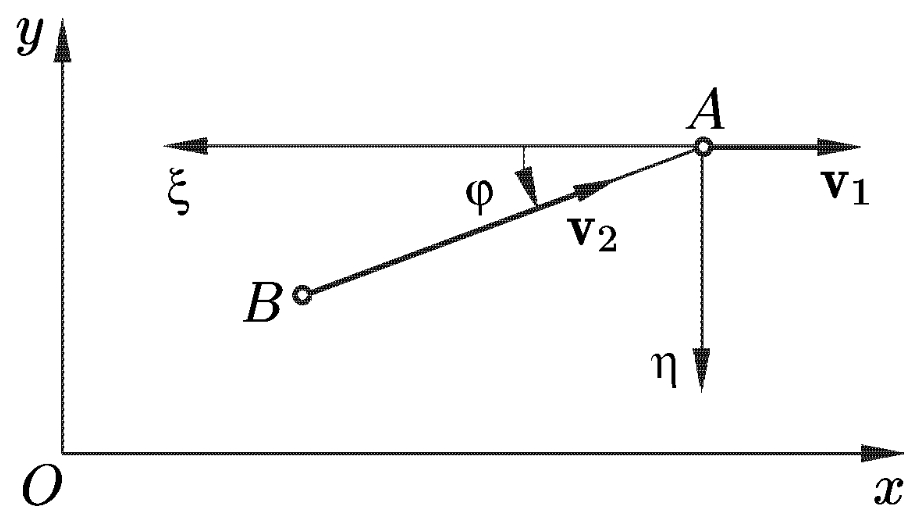
\includegraphics[width=5cm]{1-29}
\end{wrapfigure}
\paragraph{1.29.} Самолёт, изображённый на~рисунке точкой~$A$,
движется горизонтально на~высоте~$H$ с~постоянной скоростью
$\vec v_1 = \vec v$. В~момент, когда самолёт пролетает над~ракетной
установкой, пускают самонаводящуюся ракету~$B$, имеющую скорость
$\vec v_2$ и~всё время направленную к~точке~$A$, $\abs{\vec v_2} =
2\abs{\vec{v}}$. Найти уравнение траектории ракеты $AB = r(\varphi)$
в~системе отсчёта~$A\xi\eta$, движущейся вместе с~самолётом.
Найти также время полёта ракеты с~момента вылета до~поражения
самолёта и~её ускорение как~функцию угла~$\varphi$.

$\blacktriangleright$ Радиальная и~трансверсальная скорости
ракеты равны по~модулю соответствующим проекциям относительной
скорости $(\vec v_2 - \vec v_1)$ вдоль и ортогонально~$AB$:
\begin{align}
    v_r &= -v_2 + v_1 \cos\varphi = -(2 - \cos\varphi)v,
        \label{1.29:vr}\\
    v_\varphi &= -v_1 \sin\varphi = -v \sin\varphi. \label{1.29:vphi}
\end{align}
Компоненты скорости в~полярной системе координат известны:
вводя в систему уравнения~\eqref{1.20:vr} и~\eqref{1.20:vphi},
получим
\begin{gather}
\begin{cases}
    \dfrac{dr}{dt} = -(2 - \cos\varphi) v, \\[3mm]
    \dfrac{d\varphi}{dt} = -\dfrac{v \sin\varphi}{r}
\end{cases} \Longrightarrow \quad
    \frac{dr}{r} = \frac{2-\cos\varphi}{\sin\varphi}\,d\varphi.
        \label{1.29:deq}
\end{gather}
Последнее дифференциальное уравнение легко интегрируется:
\begin{align}
\tag*{\footnotesize(\ref{1.29:deq}$^\text{A}$)}
    &\int \frac{dr}{r} = \ln r + \const; \\
\tag*{\footnotesize(\ref{1.29:deq}$^\text{B}$)}
    &\int \frac{d\varphi}{\sin\varphi}
    = \int \frac{d\varphi}{\sin\frac{\varphi}{2}\cos\frac{\varphi}{2}}
    = \int \frac{\cos\frac{\varphi}{2}}{\sin\frac{\varphi}{2}}
    \frac{d\left(\frac{\varphi}{2}\right)}{\cos^2\frac{\varphi}{2}}
    = \int \frac{d\tan\frac{\varphi}{2}}{\tan\frac{\varphi}{2}}
    = \ln\tan\frac{\varphi}{2} + \const; \\[2mm]
\tag*{\footnotesize(\ref{1.29:deq}$^\text{C}$)}
    &\int \frac{\cos\varphi\,d\varphi}{\sin\varphi}
    = \frac{d\sin\varphi}{\sin\varphi} = \ln\sin\varphi + \const.
        \\[1ex]
    &r = C_1 \frac{\tan^2\frac{\varphi}{2}}{\sin\varphi}
    = C_1 \frac{\sin\varphi}{\left( 1 + \cos\varphi \right)^2}.
        \label{1.29:r}
\end{align}
Константу интегрирования найдём из~начального условия
$r\!\left(\dfrac{\pi}{2}\right) = H = C_1$.

Для~нахождения времени заметим, что при~$r \to 0$
полярный угол $\varphi \to 0$;
\begin{align}
    \dd{\varphi}{t} = -\frac{v}{H} \left(1+\cos\varphi\right)^2 \then
    \frac{d\varphi}{\left(1+\cos\varphi\right)^2} = -\frac{v\,dt}{H}.
        \label{1.29:deq2}
\end{align}
Очередное дифференциальное уравнение также интегрируется:
\begin{align}
\tag*{\footnotesize(\ref{1.29:deq2}$^\text{A}$)}
\begin{split}
    \int \frac{d\varphi}{\left(1+\cos\varphi\right)^2}
        &= \frac{1}{2} \int \frac{d\left(\frac{\varphi}{2}\right)}
            {\cos^4 \frac{\varphi}{2}}
        = \frac{1}{2} \int \frac{1}{\cos^2 \frac{\varphi}{2}}
            \frac{d\left(\frac{\varphi}{2}\right)}
            {\cos^2 \frac{\varphi}{2}} = \\
        &= \frac{1}{2} \int \left(1 + \tan^2 \frac{\varphi}{2}\right)
            d\tan\frac{\varphi}{2}
        = \frac{1}{2}\tan\frac{\varphi}{2} +
            \frac{1}{6}\tan^3\frac{\varphi}{6} + C_2.
\end{split} \\[1ex]
    t &= -\frac{H}{v} \left( \frac{1}{2}\tan\frac{\varphi}{2} +
            \frac{1}{6}\tan^3\frac{\varphi}{6} + C_2 \right)\!.
\end{align}
С~учётом $t\!\left(\dfrac{\pi}{2}\right) = 0$ найдём
очередную константу дифференцирования $C_2 = -\dfrac{2}{3}$.
Таким образом, искомое время полёта ракеты
\begin{equation}
    T = t(0) = \frac{2H}{3v}.
\end{equation}

Определим компоненты ускорения при~помощи~\eqref{1.20:wr}
и~\eqref{1.20:wphi} с~учётом \eqref{1.29:vr}, \eqref{1.29:vphi}
и~\eqref{1.29:r}:
\begin{align}
    w_r &= \ddot r - r \dot\varphi^2 = -v \sin\varphi \cdot
            \left(-\frac{v \sin\varphi}{r}\right) -
            \frac{v^2 \sin^2\varphi}{r} = 0; \\
\begin{split}
    w_\varphi &= r \ddot\varphi + 2 \dot r \dot\varphi
        = \dd{(r \dot\varphi)}{t} + \dot r \dot\varphi
        = -v \cos\varphi \cdot \dot\varphi +
            (\cos\varphi - 2) v \cdot \dot\varphi \\
        &= -2v \dot\varphi = \frac{2v^2 \sin\varphi}{r}
        = \frac{2v^2}{H} \left( 1 + \cos\varphi \right)^2.
\end{split}
\end{align}

\textbf{Ответ:}\quad
$r(\varphi) =
    \dfrac{H \sin\varphi}{\left( 1 + \cos\varphi \right)^2}$;\qquad
$T = \dfrac{2H}{3v}$;\qquad
$w(\varphi) = \dfrac{2v^2}{H} \left(1 + \cos\varphi\right)^2$.
\hfill $\blacktriangleleft$


\paragraph{1.37(б).} Найти скорость точки и~проекции её
ускорения на~касательные к~координатным линиям
для~сферических координат $r, \theta, \varphi$:
\begin{equation}
    \begin{cases}
        x = r\sin\theta\cos\varphi, \\
        y = r\sin\theta\sin\varphi, \\
        z = r\cos\theta.
    \end{cases}
\end{equation}

$\blacktriangleright$ Сначала найдём коэффициенты Ламе
данной координатной системы:
\begin{align}
    H_r &= \sqrt{\left(\pdd{x}{r}\right)^2 +
            \left(\pdd{y}{r}\right)^2 +
            \left(\pdd{z}{r}\right)^2}
        = \sqrt{\sin^2\theta \cos^2\varphi +
            \sin^2\theta \sin^2\varphi +
            \cos^2\theta} = 1; \\
    H_\theta &= \sqrt{r^2 \cos^2\theta \cos^2\varphi +
            r^2 \cos^2\theta \sin^2\varphi +
            r^2 \sin^2\theta} = r; \\
    H_\varphi &= \sqrt{r^2 \sin^2\theta \sin^2\varphi +
            r^2 \sin^2\theta \cos^2\varphi} = r \sin\theta.
\end{align}
Квадрат модуля скорости точки в~таком случае есть
\begin{equation}
    v^2 = \dot r^2 + r^2 \dot\theta^2 +
            r^2 \sin^2\theta \cdot \dot\varphi^2;
\end{equation}
компоненты ускорения рассчитываются аналогично~\eqref{1.20:wr}:
\begin{align}
    w_r &= \frac{1}{2} \left[ \dd{}{t}
            \left( \pdd{v^2}{\dot r} \right) -
            \pdd{v^2}{r} \right]
        = \ddot r - r \left( \dot\theta^2 +
            \dot\varphi^2 \sin^2\theta \right)\!, \\
    w_\theta &= \frac{1}{r} \left[ \dd{(r^2 \dot\theta)}{t} -
            r^2 \sin\theta \cos\theta \cdot \dot\varphi^2 \right]
        = r \ddot\theta + 2\dot\theta \dot r -
            r \dot\varphi^2 \sin\theta \cos\theta, \\
    w_\varphi &= \frac{1}{r\sin\theta}
            \dd{(r^2 \dot\varphi \sin^2\theta)}{t}
        = (2 \dot r \dot\varphi + r \ddot\varphi) \sin\theta +
            2r \dot\varphi \dot\theta \cos\theta.
\end{align}

\textbf{Ответ:}\quad
$v = \sqrt{\dot r^2 + r^2 \dot\theta^2 +
    r^2 \dot\varphi^2 \sin\theta^2}$;\qquad
$w = \begin{pmatrix}
    \ddot r - r \left( \dot\theta^2 +
            \dot\varphi^2 \sin^2\theta \right) \\
    r \ddot\theta + 2\dot\theta \dot r -
            r \dot\varphi^2 \sin\theta \cos\theta \\
    (2 \dot r \dot\varphi + r \ddot\varphi) \sin\theta +
            2r \dot\varphi \dot\theta \cos\theta
\end{pmatrix}$.
\hfill $\blacktriangleleft$

\clearpage

\paragraph{1.41.} Точка движется по~поверхности сферы вдоль
координатной линии сферической системы координат
$\varphi (r=\const, \theta=\const)$ с~постоянной скоростью~$v$.
Найти вектор кривизны траектории и~указать условия, при~которых
траектория точки является геодезической.

$\blacktriangleright$ При~решении настоящей задачи удобно
воспользоваться ранее полученными в~1.37(б) результатами:
\begin{equation}
    \vec v = \vec v_r + \vec v_\theta + \vec v_\varphi
        = \dot r\,\mathbf{e_r} + r\dot\theta\,\mathbf{e_\theta} +
            r \dot\varphi \sin\theta\,\mathbf{e_\varphi}.
\end{equation}
Поскольку точка движется вдоль координатной линии $\varphi$,
производные $\dot r$ и $\dot\theta = 0$, следовательно,
векторы скорости и ускорения имеют разложения
\begin{align}
    \vec v &= r \dot\varphi \sin\theta\,\mathbf{e_\varphi}; \\
    \vec w &= - r \dot\varphi^2 \sin^2\theta\,\mathbf{e_r} -
            r \dot\varphi^2 \sin\theta
                \cos\theta\,\mathbf{e_\theta} +
            (2 \dot r \dot\varphi + r \ddot\varphi) \sin\theta
                \,\mathbf{e_\varphi}.
\end{align}
Таким образом, базисный орт $\mathbf{e_\varphi}$ играет роль
касательного вектора к траектории точки. Тогда нормальная
компонента ускорения лежит в~плоскости
$\left<\mathbf{e_r}, \mathbf{e_\theta}\right>$;
вектор кривизны найдём делением последней на~квадрат скорости:
\begin{align}
    \vec{\omega_n} &= -r \dot\varphi^2 \sin\theta
            \left( \sin\theta\,\mathbf{e_r} +
            \cos\theta\,\mathbf{e_\theta} \right); \\
    \vec{k} &= \frac{\vec\omega_n}{v^2}
        = -\frac{\sin\theta\,\mathbf{e_r} +
            \cos\theta\,\mathbf{e_\theta}}{r \sin\theta}
        = -\frac{1}{r} \left( \mathbf{e_r} +
            \frac{\mathbf{e_\theta}}{\tan\theta} \right).
\end{align}

Траектория точки является геодезической, если $\vec k$
направлен по~нормали к поверхности сферы $r = \const$,
а~стало быть~--- ортогонален $\mathbf{e_\theta}$
и~$\mathbf{e_\varphi}$, что требует нулевых коэффициентов
при~упомянутых ортах в~разложении~$\vec k$
($\tan\theta \to \infty$).

\textsl{Примечание.} Данное рассуждение подтверждает
геометрически интуитивную идею о~том, что геодезическая параллель
на~сфере, большой круг с~$\theta = \const$~--- это экватор.

\textbf{Ответ:}\quad
$\vec k = -\dfrac{1}{r} \left( \mathbf{e_r} +
    \dfrac{\mathbf{e_\theta}}{\tan\theta} \right)$;\qquad
при~условии $\theta = \dfrac{\pi}{2}$.
\hfill $\blacktriangleleft$

\end{document}
